% !TEX encoding = UTF-8 Unicode
\documentclass[a4paper]{article}

\usepackage{color}
\usepackage{url}
\usepackage[T2A]{fontenc} % enable Cyrillic fonts
\usepackage[utf8]{inputenc} % make weird characters work
\usepackage{graphicx}
\usepackage{amsmath}
\usepackage[english,serbian]{babel}
%\usepackage[english,serbianc]{babel} %ukljuciti babel sa ovim opcijama, umesto gornjim, ukoliko se koristi cirilica

\usepackage[unicode]{hyperref}
\hypersetup{colorlinks,citecolor=green,filecolor=green,linkcolor=blue,urlcolor=blue}

\usepackage{listings}

%\newtheorem{primer}{Пример}[section] %ćirilični primer
\newtheorem{primer}{Primer}[section]

\definecolor{mygreen}{rgb}{0,0.6,0}
\definecolor{mygray}{rgb}{0.5,0.5,0.5}
\definecolor{mymauve}{rgb}{0.58,0,0.82}

\lstset{ 
  backgroundcolor=\color{white},   % choose the background color; you must add \usepackage{color} or \usepackage{xcolor}; should come as last argument
  basicstyle=\scriptsize\ttfamily,        % the size of the fonts that are used for the code
  breakatwhitespace=false,         % sets if automatic breaks should only happen at whitespace
  breaklines=true,                 % sets automatic line breaking
  captionpos=b,                    % sets the caption-position to bottom
  commentstyle=\color{mygreen},    % comment style
  deletekeywords={...},            % if you want to delete keywords from the given language
  escapeinside={\%*}{*)},          % if you want to add LaTeX within your code
  extendedchars=true,              % lets you use non-ASCII characters; for 8-bits encodings only, does not work with UTF-8
  firstnumber=1000,                % start line enumeration with line 1000
  frame=single,	                   % adds a frame around the code
  keepspaces=true,                 % keeps spaces in text, useful for keeping indentation of code (possibly needs columns=flexible)
  keywordstyle=\color{blue},       % keyword style
  language=Python,                 % the language of the code
  morekeywords={*,...},            % if you want to add more keywords to the set
  numbers=left,                    % where to put the line-numbers; possible values are (none, left, right)
  numbersep=5pt,                   % how far the line-numbers are from the code
  numberstyle=\tiny\color{mygray}, % the style that is used for the line-numbers
  rulecolor=\color{black},         % if not set, the frame-color may be changed on line-breaks within not-black text (e.g. comments (green here))
  showspaces=false,                % show spaces everywhere adding particular underscores; it overrides 'showstringspaces'
  showstringspaces=false,          % underline spaces within strings only
  showtabs=false,                  % show tabs within strings adding particular underscores
  stepnumber=2,                    % the step between two line-numbers. If it's 1, each line will be numbered
  stringstyle=\color{mymauve},     % string literal style
  tabsize=2,	                   % sets default tabsize to 2 spaces
  title=\lstname                   % show the filename of files included with \lstinputlisting; also try caption instead of title
}

\begin{document}

\title{Genetski algoritam za višeciljnu optimizaciju\\ }

\author{Aleksandra Bošković, Miloš Miković\\ aleksandra94@hotmail.rs, milos.mikovicpos@gmail.com}

%\date{9.~april 2015.}

\maketitle

\tableofcontents

\newpage

\section{Uvod}
\label{sec:uvod}

Problem trgovačkog putnika (Traveling Salesman Problem, TSP) je jedan od najpoznatijih  problema iz grupe NP - teških problema diskretne i kombinatorne optimizacije.U osnovi ovaj problem je definisan na sledeći način: trgovački putnik tačno zna koje gradove treba da poseti i koja je njihova međusobna udaljenost, jedini problem je što je u obavezi da poseti svaki grad samo jednom i vrati se u grad iz kog je krenuo. Ovom osnovnom problemu dodaćemo jos jedan podatak koji trgovački putnik ima a to je vreme potrebno da se pređe put između svaka dva grada. Cilj je pronaći tačnu putanju kojom trgovački putnik treba da ide tako da i ukupno provedeno vreme na putu i ukupna pređena dužina puta budu minimalni. Ovu putanju ćemo pokušati da pronađemo korišćenjem genetskog algoritma.
\par
Ideja zasnovana na idejama iz literature \cite{2} , \cite{3} i \cite{4}



\section{Algoritam}
\\
\textbf{Ulaz:} podaci o udaljenosti između svakog od gradova, kao i potrebno vreme za prelazak puta između svakog od gradova
\\
\textbf{Izlaz:} najbolje pronađeno rešenje genetskim algoritmom
\\
\\
Da bismo mogli da poredimo rešenja definišimo prvo funkciju cilja za ovaj problem:
\[ 
  \begin{cases}
    min \sum_{i=1,j=1}^{n,n} d_i_j ,  \\
    min \sum_{i=1,j=1}^{n,n} t_i_j\\
  \end{cases}
\]
gde je $d_i_j$ dužina puta od grada $i$ do grada $j$, a $t_i_j$ veme potrebno da se pređe put od grada $i$ do grada $j$.\par
Sa obzirom na to da je često nemoguće u isto vreme minimizovati obe funkcije, a u cilju podjednakog vrednovanja obe veličine definišimo funkciju cilja na sledeći način
$$ f(x)=\frac{D_x}{\sum_{i=1}^{m} D_i} + \frac{T_x}{\sum_{i=1}^{m} T_i}$$
pri čemu je $m$ broj jedinki u generaciji $D_x$ ukupna dužina pređenog puta za rešenje $x$ a $T_x$ ukpno vreme potrebno da se pređe odabrani put $x$.\par
Naš cilj je da za odabrano rešenje $x$ važi:
$$f(x)<f(x') , \forall x' \in \Omega $$
pri čemu je $\Omega$ skup svih permutacija skupa gradova kroz koje putnik treba da prođe a $x$ izabrana najbolja permutacija.\par
\newpage
\subsection{Opis implementacije elemenata genetskog algoritma}
\textbf{Kodiranje jedinke:}\\ predstavljena je kao permutacija skupa svih gradova i predstavlja redosled kojim trgovački putnik obilazi gradove.\\
\textbf{Inicijalna populacija:}\\ generisana je random iz skupa svih mogućih permutacija obilaska gradova. \\
\textbf{Selekcija:}\\
turnirska selekcija odabira jedinki za ukrštanje.\\
\textbf{Mutacija:} \\zamena random odabrana dva indeksa niza koji predstavlja jedinku \cite{1}.\\
\textbf{Ukrštanje:}\\ 
\textit{Prvi način:} ukrštanje prvog reda za kombinatorne probleme\\
\textit{Drugi način:} random odabran segment jednog roditelja staviti na početak deteta a ostatak niza dopuniti preostalim elementima onim redosledom kojim se javljaju u drugom roditelju. \\
Drugi način se pokazao kao bolji jer prvi prebrzo konvergira.\\
\textbf{Nova populacija:} \\n odabranih najboljih jedinki iz prethodne generacije i deca ukrštenih roditelja.
\textbf{Kriterijum zaustavljanja:}\\ dostignut zadati broj iteracija.

\section{Poređenje sa brute force algoritmom}
U cilju ocenjivanja dobijenog rešenja ovakvim algoritmom uporedimo sa rešenjem dobijenim brute force algoritmom, koji ispituje sve moguće permutacije.U algoritmu brute force pri odabiru najboljeg rešenja tražimo minimum funkcje:
$$ f(x)=\frac{D_x}{\sum_{i=1}^{n!} D_i} + \frac{T_x}{\sum_{i=1}^{n!} T_i}$$
pri čemu su korišćene oznake iste kao i kog rešenja za genetski algoritmom. Uočimo razliku da ovde u imeniocu sumiramo vrednosti svih mogućih permutacija jer su nam one poznate, dok nam kod rešenja genetskim algoritmom ova suma zavisi od populacije u svakoj generaciji.\par
U nastavku na slikama su dati rezultati posmatranog problema za 11 gradova, 100 generacija, verovatnoćom mutacije 0.05, veličinom generacije 20, veličinom turnira 5. Pri čemu najbolje rešenje koje pronalazi algoritam brute force za ovih 11 gradova iznosi $D=29$ za ukupnu dužinu optimalnog puta i $T=32$ za vreme potrebno da se pređe optimalan put.

\newpage
Na slici \ref{fig:pande} možemo pratiti na koji način se izabrana vrednost optimalnog rešenja u svakoj generaciji menja i približava vrednosti koji je pronašao algoritam brute force za dužinu puta.

\begin{figure}[h!]
\begin{center}
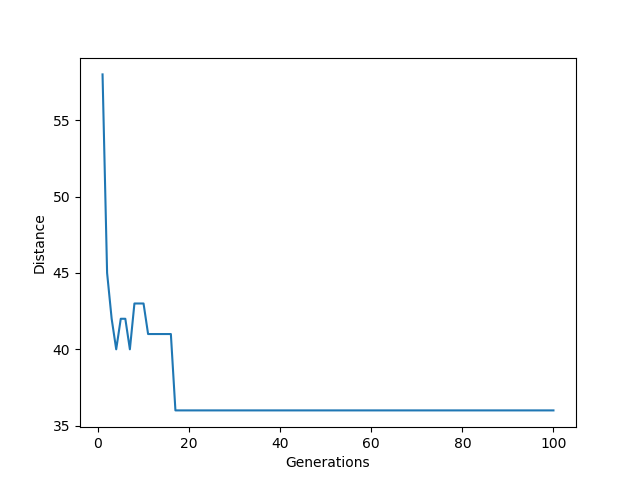
\includegraphics[scale=0.40]{1.png}
\end{center}
\caption{Dužina puta izabranog optimalnog rešenja kroz generacije}
\label{fig:pande}
\end{figure}

Na slici \ref{fig:pande2} možemo pratiti na koji način se izabrana vrednost optimalnog rešenja u svakoj generaciji menja i približava vrednosti koji je pronašao algoritam brute force za vreme potrebno da se pređe optimalan put.
\begin{figure}[h!]
\begin{center}
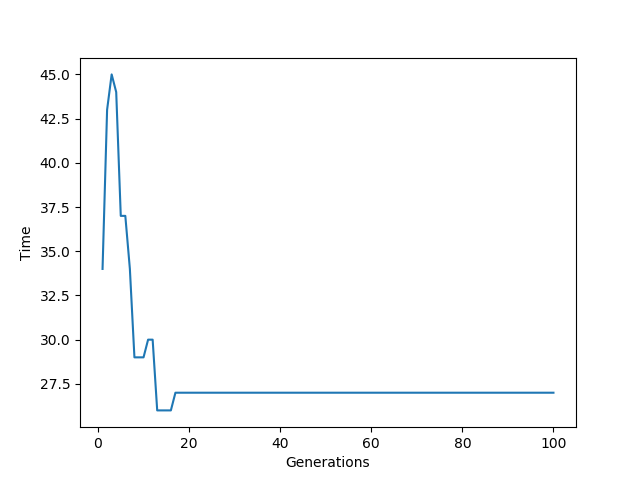
\includegraphics[scale=0.40]{2.png}
\end{center}
\caption{Vreme potrebno da se pređe optimalan put kroz generacije}
\label{fig:pande2}
\end{figure}
\newpage
Slika \ref{fig:pande3} objedinjuje prethodne slike i prikazuje vrednosti obe dimenzije problema kroz generacije
\begin{figure}[h!]
\begin{center}
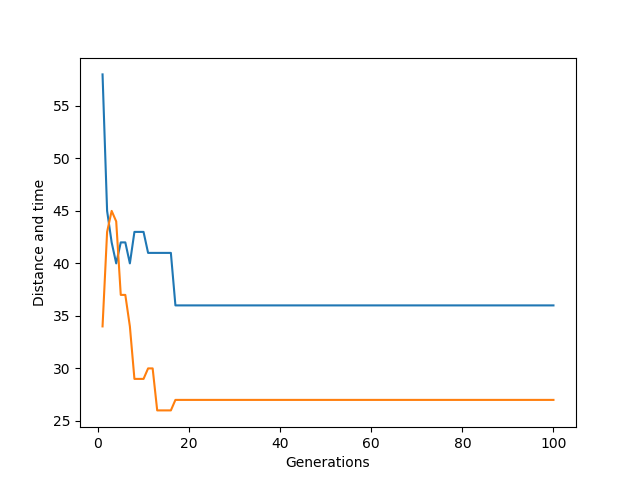
\includegraphics[scale=0.60]{3.png}
\end{center}
\caption{Optimalno rešenje kroz generacije}
\label{fig:pande3}
\end{figure}

Na sledećim tabelama prikazaćemo na primeru 11(tabela \ref{tab:tabela1}) i 10(tabela \ref{tab:tabela2}) gradova procenat da predloženi genetski algoritam za optimalno rešenje dobije neki od najboljih 5 rešenja dobijenih algoritmom brute force.

\begin{table}[h!]
\begin{center}
\caption{Vrednosti u tabeli važe za posmatran problem 11 gradova, veličinom populacije 20, verovatnoćom mutacije 0.05,veličinom turnira 5 i brojem generacija 3000}
\begin{tabular}{|c|c|c|} \hline
Distanca& Vreme & Odabran za optimalno\\ \hline
 29& 32& 27\%\\ \hline
 33& 29& 0\%\\ \hline
 32& 30& 46\%\\ \hline
 36& 27& 0\%\\ \hline
 33& 30& 0\%\\ \hline
\end{tabular}
\label{tab:tabela1}
\end{center}
\end{table}

\begin{table}[h!]
\begin{center}
\caption{Vrednosti u tabeli važe za posmatran problem 10 gradova, veličinom populacije 20, verovatnoćom mutacije 0.05,veličinom turnira 5 i brojem generacija 2500}
\begin{tabular}{|c|c|c|} \hline
Distanca& Vreme & Odabran za optimalno\\ \hline
 30& 29& 17\%\\ \hline
 23& 35& 18\%\\ \hline
 26& 33& 32\%\\ \hline
 32& 28& 0\%\\ \hline
 27& 33& 0\%\\ \hline
\end{tabular}
\label{tab:tabela2}
\end{center}
\end{table}
\newpage
Svi testovi rađeni su na računaru sledećih karakteristika:\\
Operativni sistem: GNU/Linux\\
Procesor: Intel i7-6498DU 2.50ghz\\
Ram memorija: 8GB\\


\section{Zaključak}
Prikazani genetski algoritam na problemu trgovačkog putnika sa dodatim zahtevima za vreme može pronaći globalno optimalno rešenje sa velikom verovatnoćom. U cilju poboljšanja ovog algoritma moguće je inicijalnu populaciju generisati pažljivim odabirom permutacija, tako da pri konstrukciji permutacije gradove navodimo tako da njihova međusobna udaljenost ili vreme budu što je moguće manji \cite{3}.Ova poboljšanja u vidu inicijalne populacije mogu povećati vreme izvršavanja algoritma, ali su tačniji.
\label{sec:zakljucak}

\newpage

\addcontentsline{toc}{section}{Literatura}
\appendix
\bibliography{seminarski} 
\bibliographystyle{plain}

\appendix

\end{document}